\begin{figure}
	\centering
	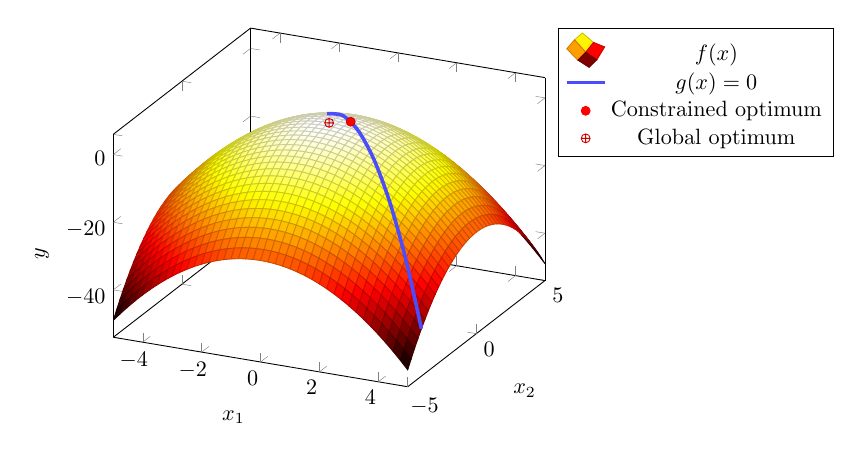
\begin{tikzpicture}[
		scale=0.8
	]

		\begin{axis}[
			legend pos=outer north east,
			xlabel={$x_1$},
    			ylabel={$x_2$},
    			zlabel={$y$}
		]

			\addplot3[
				surf,
				colormap/hot2,
				samples=41
			] {1-x^2-y^2};

			\addplot3[
				ultra thick,
				samples y=1,
				blue!70,
				smooth
			] table[z expr=1-x^2-y^2]
    			{
        			x  y
				5 -4
				4  -3
				3  -2
				2  -1
				1  0
				0  1
				-1  2
    			};
    				
			\addplot3[
				scatter,
				only marks,
				red
			] table[z expr=1-x^2-y^2]
			{
				x  y
				0.5  0.5
			};

			\addplot3[
				scatter,
				only marks,
				mark=oplus,
				red!80!black
			] table[z expr=1-x^2-y^2]
			{
				x  y
				0  0
			};

			\legend{$f(\bm{x})$, $g(\bm{x}) = 0$, Constrained optimum, Global optimum}
		\end{axis}
		
	\end{tikzpicture}
\end{figure}